
\section{Project 1: Basic Statistics with Hadoop Cloud Computing
  Spring 2017}       

Judy Qiu

\section*{Problem statement}
 
The idea of this project is to get you started with Hadoop and the MapReduce concept. You may have already looked at the WordCount example, both serial and Hadoop implementations. This problem is similar to WordCount except that you will be computing the basic statistics such as min, max, average, and standard deviation of a given data set.

The input to the program will be a text file carrying exactly one floating point number per line. The output should include \textbf{min, max, average, and standard deviation} of these numbers.

\begin{figure}[!htbp]
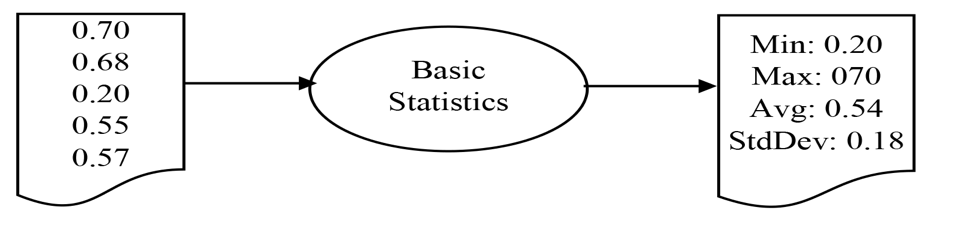
\includegraphics[width=8cm,height=3cm]{section/icloud/assignment/problems/project1/p1example.png}
\centering
\end{figure}

\section*{Files}
A test input file is available as a separate attachment.
The statistics values for this input are \textbf{Min: 0.01 Max: 0.99 Avg: 0.50 StdDev: 0.2817}


\section*{Deliverables}
You will need to complete the source code and write a report. Zip your work into a file with the name username\_project1.zip (replace 'username' with your own) and submit the following:
\begin{itemize}
\item Complete source code
\item A document with the following details:
\begin{itemize}
\item	Transformation of data during the computations, i.e. data type of key, value
\item	The data structure used to transfer between Map and Reduce phases
\item	How the data flow happens through disk and memory during the computation
\end{itemize}
\end{itemize}

\section*{Evaluation}
The point total for this project is 5.
\begin{itemize}
\item Correctness of the source code (2 points)
\item	Completeness of the report (3 points)
\end{itemize}

